\documentclass{article}
% --- watermark (auto-inserted) ---
\usepackage{xcolor}
\usepackage{xfp}% \fpeval; in the kernel since 2022, harmless on older LaTeX
\usepackage{draftwatermark}
\newlength{\watermarkTextWidth}
\AddToHook{begindocument/end}{%
  \SetWatermarkText{\normalfont Generated by The Agentic Scientist}%
  \SetWatermarkFontSize{10pt}%
  \SetWatermarkLightness{0.85}%
  \settowidth{\watermarkTextWidth}{\normalfont\fontsize{10pt}{12pt}\selectfont Generated by The Agentic Scientist}%
  \edef\watermarkScale{\fpeval{0.8 * sqrt(\paperwidth**2 + \paperheight**2) / \watermarkTextWidth}}%
  \edef\watermarkAngle{\fpeval{atand(\paperheight/\paperwidth)}}%
  \SetWatermarkScale{\watermarkScale}%
  \SetWatermarkAngle{\watermarkAngle}%
}
% --- end watermark ---
\usepackage{source_evidence/iclr2026_conference,times}
\usepackage[T1]{fontenc}
\usepackage[utf8]{inputenc}
\usepackage{amsmath,amssymb,booktabs,graphicx,subcaption}
\usepackage{hyperref,url}
\newcommand{\gate}{\tau}
\newcommand{\R}{\mathbb{R}}
\title{Endpoint-Tuned Regression under Network Interference: Accuracy and Limits}
\author{}
\begin{document}
\maketitle

\begin{abstract}
Regression can estimate the effect of treating an entire network by predicting outcomes under all-treated and all-control assignments. However, fitting observed outcomes and estimating this intervention contrast are different statistical objectives. We study a one-hop exposure regression that tunes ridge regularization using an endpoint-contrast risk criterion, comparing it with difference in means, own-treatment regression, and linear one-hop regression. A fixed evaluation comprises 24 seed blocks, four network families, and six interference/design conditions, including synthetic outcomes on Stanford3. The endpoint-tuned estimator has mean cell RMSE 0.614, compared with 1.368 for difference in means but 0.460 for one-hop ordinary least squares. The paired RMSE disadvantage relative to one-hop regression is 0.154, with a 95\% seed-block bootstrap interval of [0.127, 0.179]. Threshold and omitted two-hop spillovers produce substantial endpoint errors despite near-unit observed-fit residuals. These results support a conditional accuracy study, not superiority of target-aware tuning: regression specification, assignment design, and the distinction between observed support and endpoint prediction remain consequential limitations.
% @evidence[[analysis/summary.json]] @evidence[[paper_data.json#/final_evaluation/evaluation_evidence/episodes]]
\end{abstract}

\section{Introduction}
Randomized experiments on connected populations have an estimand problem as well as an estimation problem. An individual assigned to control can still be affected by treated neighbors. Consequently, a contrast between the observed treatment arms need not estimate what a platform would obtain by treating everyone rather than no one. Potential-outcome formulations make the intervention explicit \citep{Neyman1990,Rubin1974}; under interference, the outcome must depend on a vector of assignments rather than only the individual's assignment \citep{Hudgens2008,Manski2013}. Network experimentation at scale makes this distinction practically relevant \citep{Karrer2021}.

A natural response is to regress outcomes on treatment, covariates, and summaries of neighbors' assignments, and evaluate the fitted function at the two global interventions \citep{Chin2019}. This approach separates observed experimental data from the intervention of interest, but introduces a delicate extrapolation problem. A model can predict outcomes accurately near the observed treatment saturation while predicting the difference between saturation extremes poorly. Conversely, restricting a regression to a correctly specified low-dimensional exposure model can be more effective than adding flexible terms and regularization. Model complexity is not automatically useful for the target contrast.

We examine whether tuning regularization toward the endpoint contrast is sufficient to make a richer one-hop regression competitive. The estimator uses a quadratic exposure reference and a finite ridge grid. Its risk criterion is motivated by a fixed-design linear-model calculation, not by a general identification result. The comparison is deliberately anchored to meaningful simple alternatives: difference in means, covariate-adjusted own-treatment regression, and linear one-hop ordinary least squares (OLS). The scientific question is how their errors change across network structures, interference mechanisms, and assignment designs, rather than whether a single aggregate evaluation measure is high.

The evidence yields a negative answer to general superiority. Across the fixed benchmark, endpoint tuning substantially reduces aggregate error relative to assignment-only analysis but loses to linear one-hop OLS. The latter comparison is essential: a gain over a baseline that omits spillovers is not evidence that a more elaborate exposure regression is preferable. Threshold and two-hop conditions also show that small residuals on observed assignments do not certify accurate global intervention prediction.

Our contributions are a concrete endpoint-functional tuning construction, a matched comparison across the complete recorded condition matrix, and an analysis of its observed limitations. We report Monte Carlo uncertainty at the seed-block level and distinguish it from causal confidence-interval coverage. Because feature expansion and tuning are not separately ablated, the results compare complete estimators; they do not attribute error differences to the tuning objective alone. Figure~\ref{fig:overview} summarizes the distinction that organizes the study.

\begin{figure}[t]
\centering

\includegraphics[width=.98\textwidth]{figures/endpoint_overview.png}
\caption{The target is an intervention contrast, not observed prediction error. A graph, covariates, observed assignment, and observed outcomes determine the fitted regression. All-treated and all-control assignments are separate prediction inputs; their outcomes are withheld from fitting. Algebraic estimability of the fitted contrast does not establish exposure support or robustness to misspecification.}
\label{fig:overview}
\end{figure}

\section{Related Work}
\paragraph{Interference and experimental design.}
\citet{Aronow2017} distinguish the assignment design, exposure mapping, and causal estimand in a randomization-based framework. Graph cluster randomization changes exposure probabilities and can improve design-based estimation under suitable exposure assumptions \citep{Ugander2013}. Design and analysis can both reduce interference bias without eliminating the dependence on modeling assumptions \citep{Eckles2017}. Staggered rollout provides another route under low-order interaction assumptions without requiring the graph \citep{Cortez2022}. These are distinct designs and inferential targets; our static assignment comparisons do not evaluate their complete estimators or variance guarantees.

\paragraph{Regression adjustment.}
Global intervention prediction from regression is established by \citet{Chin2019}. Graph- and treatment-based covariate generation and selection, together with block-bootstrap inference, are studied by \citet{Han2023}. We do not introduce regression adjustment for interference or compare against that full covariate-selection procedure. Instead, we evaluate a small, explicitly specified one-hop reference. The broader regression-adjustment literature cautions against treating model fitting as automatically beneficial \citep{Freedman2008}; favorable asymptotic results require attention to interactions and variance estimation \citep{Lin2013}. Those results under individualistic response cannot be transferred directly to the present endpoint-extrapolation setting.

\paragraph{Regularization and assessment.}
Ridge regression addresses unstable estimation with correlated predictors \citep{Hoerl1970}. Generalized cross-validation targets prediction through a rotation-invariant criterion \citep{Golub1979}. Unbiased risk estimation motivates target-specific assessment \citep{Stein1981}, but apparent error can be optimistic when the same data are used for fitting and evaluation \citep{Efron1986}. We distinguish a fixed-penalty identity from the selected minimum. Estimable linear functions are a linear-algebraic notion \citep{Searle1965}; neither estimability nor heteroskedasticity-consistent variance estimation \citep{White1980} alone addresses a missing spillover mechanism. Our bootstrap summarizes repeated experimental realizations \citep{Efron1979}, not unmeasured inferential coverage. Finally, the graph families represent block structure \citep{Choi2012}, preferential attachment \citep{Barabasi1999}, small-world structure \citep{Watts1998}, and a public social-network topology \citep{Traud2012,Rossi2015}; they are not a random sample of online platforms.

\section{Method}
\subsection{Problem Setup and Design Rationale}
For an undirected graph with adjacency matrix $A$, let $d_i=\sum_j A_{ij}$ and define the one-hop exposure and length-two exposure by
\begin{equation}
e_i(z)=\frac{\sum_j A_{ij}z_j}{\max(d_i,1)},\qquad
h_i(z)=\frac{\sum_j A_{ij}e_j(z)}{\max(d_i,1)}.
\label{eq:exposure}
\end{equation}
The second expression averages neighbors' exposures and includes backtracking walks; it is not the fraction of distinct distance-two neighbors treated. Isolates retain exposure zero. Given fixed covariates and a fixed noise realization, the finite-population target is
\begin{equation}
\gate=\frac{1}{n}\sum_i\{Y_i(\mathbf{1})-Y_i(\mathbf{0})\},\qquad
\widehat\gate=\frac{1}{n}\sum_i\{\widehat f_i(\mathbf{1})-\widehat f_i(\mathbf{0})\}.
\label{eq:target}
\end{equation}
Only the graph, covariates $x_i$, realized treatment vector $z$, and $Y_i(z)$ are available during fitting. Endpoint outcomes and the target effect are not training feedback. We study point-estimation error, not recovery of every potential outcome.
% @evidence[[source_evidence/evaluate_final.py#L676-L694]] @evidence[[source_evidence/estimator.py#L180-L213]]

The design rationale is that regularization should account for the particular linear functional in Equation~\ref{eq:target}, rather than only average prediction near observed exposures. Our working hypothesis is conditional: an adequate and estimable reference can support endpoint-oriented bias--variance tuning. It does not imply that a richer reference improves on correctly specified one-hop OLS, or that one-hop features recover omitted multi-hop effects.

\subsection{Endpoint-Tuned Exposure Regression}
The inspected estimator source associated with the frozen evaluation constructs the reference
\begin{equation}
\phi_i(z)=\bigl[1,\ x_i^\top,\ z_i,\ e_i(z),\ z_i e_i(z),\ c_i(z),\ z_i c_i(z)\bigr],
\qquad c_i(z)=e_i(z)\{1-e_i(z)\}.
\label{eq:features}
\end{equation}
The curvature terms vanish at exposure extremes but affect the observed fit. All non-intercept columns are centered and scaled using observed-assignment means and population standard deviations. Zero scales are replaced by one. Endpoint rows use this same saved transformation; the intercept is unpenalized. The complete source is provided as \texttt{source\_evidence/estimator.py}, functions \texttt{\_reference\_features} and \texttt{\_fit\_endpoint\_sure}.
% @evidence[[source_evidence/estimator.py#L83-L160]]

Let $W$ be the standardized non-intercept design, $y_c=y-\bar y\mathbf{1}$, and $q$ the difference between the mean transformed endpoint rows. For retained singular values, write $W=USV^\top$ and $v=V^\top q$. The reference contrast and each ridge contrast have weights
\begin{equation}
a_0=US^{-1}v,\qquad a_\lambda=US(S^2+\lambda I)^{-1}v,\qquad
\widehat\gate_\lambda=a_\lambda^\top y_c.
\label{eq:weights}
\end{equation}
Here $V$ contains retained right singular vectors, so $q$ must lie in their span. The residual variance estimate is $\widehat\sigma^2=\|(I-UU^\top)y_c\|^2/(n-r-1)$, where $r$ is retained rank. The criterion is
\begin{equation}
\widehat R(\lambda)=
(\widehat\gate_\lambda-\widehat\gate_0)^2
+2\widehat\sigma^2 a_\lambda^\top a_0-\widehat\sigma^2\|a_0\|^2,
\quad
\lambda\in n\{0,10^{-6},10^{-4},10^{-2},1\}.
\label{eq:risk}
\end{equation}
The smallest criterion value is selected, with ties resolved by grid order. This is a finite observed-data rule, not access to the true endpoint error.
% @evidence[[source_evidence/estimator.py#L114-L160]]

Under a correct fixed linear reference with independent homoskedastic Gaussian errors, $a_0^\top E[y_c]=\gate$ and $E[\widehat\sigma^2]=\sigma^2$. For a \emph{fixed} penalty, the expectation of the squared difference in Equation~\ref{eq:risk} is the squared bias of $\widehat\gate_\lambda$ plus $\sigma^2\|a_\lambda-a_0\|^2$. The remaining terms convert this variance contribution to $\sigma^2\|a_\lambda\|^2$. This calculation motivates the criterion; it is not a distribution-free theorem about network effects. Choosing the smallest estimated risk does not make that minimum an unbiased estimate of the selected estimator's risk. Misspecification also invalidates the premise that the reference contrast is unbiased.

The implementation checks finite inputs and SVD output, target row-space membership, and positive residual degrees of freedom. An unusable reference falls back to a fixed-ridge one-hop hinge regression; exactly constant outcomes bypass fitting and yield zero contrast. These safeguards prevent some algebraic or behavioral failures. They do not establish endpoint support, identify arbitrary interference, or supply a causal confidence interval. Exact numerical tolerances and the fallback basis appear in Supplementary Information.
% @evidence[[source_evidence/estimator.py#L69-L81]] @evidence[[source_evidence/estimator.py#L107-L145]] @evidence[[source_evidence/estimator.py#L199-L213]]

\subsection{Compared Approaches}
Difference in means estimates the observed treated-minus-control mean outcome. Own-treatment OLS fits $[1,x_i^\top,z_i]$ and uses the treatment coefficient. One-hop OLS fits $[1,x_i^\top,z_i,e_i(z)]$ and predicts the global contrast. The latter equals the treatment coefficient plus the exposure coefficient multiplied by the fraction of nonisolated nodes. These baseline estimates are recorded on the same scientific cases as the endpoint-tuned estimator, so comparisons are paired rather than comparisons of separate simulation suites.
% @evidence[[source_evidence/evaluate_final.py#L371-L392]] @evidence[[paper_data.json#/final_evaluation/evaluation_evidence/episodes]]

No component ablation separates the quadratic reference from endpoint-risk tuning. In particular, the evidence contains no completed same-reference predictive-tuning comparison. We therefore evaluate complete configurations, not an isolated causal effect of changing the tuning objective. Constant prediction and copying observed outcomes are behavioral controls, not substantive alternatives for estimating the global effect.

\subsection{Experimental Protocol}
The fixed evaluation crosses four graph families and six conditions with 24 seed blocks, yielding 576 scientific records. Synthetic graphs have 4,096 nodes. The stochastic block model (SBM) has four blocks with within/between connection probabilities 0.04/0.002; Barab\'asi--Albert (BA) uses five attachment edges; Watts--Strogatz (WS) uses neighborhood size 10 and rewiring probability 0.15. Stanford3 is a fixed, undirected public graph with 11,586 nodes and 568,309 edges. Synthetic topologies vary across seeds; Stanford3 repeats assignments and synthetic outcomes on one topology. Covariates have one column. The recorded generator uses unit-standard-deviation Gaussian noise, held fixed across counterfactual assignments within a realization.
% @evidence[[source_evidence/benchmark_manifest.json#/generator]] @evidence[[source_evidence/benchmark_manifest.json#/records]] @evidence[[analysis/summary.json]] @evidence[[reproducibility/resources/final/benchmark.npz]]

\begin{table}[t]
\centering
\caption{Outcome and assignment conditions. All outcomes are $Y_i(z)=0.5x_i+z_i+s_i(z)+\epsilon_i$. Individual treatment is independent Bernoulli with probability $1/2$. The cluster condition changes assignment while retaining the strong-linear outcome mechanism. The recorded global effect is identical across the four families for each condition.}
\label{tab:protocol}
\begin{tabular}{llll}
\toprule
Condition & Spillover $s_i(z)$ & Assignment & $\gate$\\
\midrule
No spill & $0$ & Individual & 1\\
Weak linear & $0.25e_i$ & Individual & 1.25\\
Strong linear & $2e_i$ & Individual & 3\\
Threshold & $2\mathbf{1}\{e_i\geq0.75\}+z_i e_i$ & Individual & 4\\
Two-hop & $2h_i$ & Individual & 3\\
Cluster & $2e_i$ & Cluster & 3\\
\bottomrule
\end{tabular}
% @evidence[[source_evidence/evaluate_final.py#L686-L693]] @evidence[[source_evidence/benchmark_manifest.json#/mechanisms]] @evidence[[paper_data.json#/final_evaluation/evaluation_evidence/episodes]]
\end{table}

Table~\ref{tab:protocol} specifies the outcome mechanisms. The cluster design forms 32 deterministic graph-BFS clusters with independent cluster treatment probability $1/2$; it is not optimized for this estimator. The smallest unassigned node starts each traversal; neighbors are sorted, each cluster receives at most $\lceil n/32\rceil$ nodes, and disconnected frontiers restart at the smallest unassigned node. Assignment designs share topology, covariates, and noise within a seed/family, but this is not a controlled intervention on exposure support alone.
% @evidence[[source_evidence/benchmark_manifest.json#/mechanisms]]

We compute signed error $u_{sfkm}=\widehat\gate_{sfkm}-\gate_{sfk}$ for seed $s$, family $f$, condition $k$, and method $m$. Cell RMSE is $(S^{-1}\sum_s u_{sfkm}^2)^{1/2}$; cell absolute bias is $|S^{-1}\sum_s u_{sfkm}|$. Aggregate values average these cell summaries equally across families and conditions. This gives each condition equal scientific weight rather than weighting by node count or treating all squared errors as one pooled RMSE. Both bias and RMSE matter: a small bias may mask large dispersion, whereas systematic endpoint misspecification can dominate both.

The evaluator caps signed errors at magnitude 10 in its normalized summaries; noise scale is one. No scientific estimate was clipped, and all scientific cases completed, so the reported raw endpoint-tuned summaries equal the retained capped summaries. Missing or failed observations would not be treated as measured losses in a separate estimator comparison. No new scientific simulations were executed for this manuscript.
% @evidence[[analysis/summary.json]] @evidence[[source_evidence/benchmark_manifest.json#/aggregation]] @evidence[[paper_data.json#/final_evaluation/metrics]]

Uncertainty uses 10,000 percentile bootstrap resamples of the 24 \emph{entire seed blocks}, with resampling seed 20261107. Every draw retains all family, condition, and method observations from a chosen seed. We recompute nonlinear RMSEs and their ratios in each draw; ratios are not averages of per-seed ratios. These 95\% intervals measure Monte Carlo variability in this fixed benchmark, not unit-level causal uncertainty or generalization to a population of graphs. Condition-level intervals are exploratory and are not multiplicity-adjusted. Absolute-bias intervals are not bias-corrected.
% @evidence[[analysis/summary.json#/bootstrap]] @evidence[[build_paper_artifacts.py]]

\section{Results}
\subsection{Main Comparison: Improvement Depends on the Comparator}
Table~\ref{tab:main} gives the equal-cell accuracy summaries. The endpoint-tuned estimator's mean RMSE is 0.614, substantially below 1.368 for both assignment-only comparators, but above 0.460 for one-hop OLS. The paired difference relative to one-hop OLS is 0.154, with a 95\% bootstrap interval [0.127, 0.179]. Its mean absolute bias is also larger than that of one-hop OLS: 0.460 versus 0.393. Thus the aggregate loss is not merely a difference in the direction of signed errors that would cancel when averaged.
% @evidence[[analysis/summary.json#/rmse]] @evidence[[analysis/summary.json#/endpoint_minus_onehop_rmse_ci]] @evidence[[analysis/summary.json#/absolute_bias]]

\begin{table}[t]
\centering
\caption{Main results: mean cell RMSE and mean cell absolute bias, with 95\% paired seed-block percentile bootstrap intervals. Lower values are better. These are equal averages of cell summaries, not pooled errors over nodes or cells. Bias intervals include the nonlinearity of taking absolute seed-mean errors.}
\label{tab:main}
\begin{tabular}{lcc}
\toprule
Estimator & RMSE [95\% interval] & Absolute bias [95\% interval]\\
\midrule
Endpoint-tuned & 0.614 [0.588, 0.636] & 0.460 [0.431, 0.514]\\
Difference in means & 1.368 [1.363, 1.371] & 1.363 [1.359, 1.367]\\
Own-treatment OLS & 1.368 [1.364, 1.372] & 1.363 [1.360, 1.368]\\
One-hop OLS & 0.460 [0.445, 0.474] & 0.393 [0.391, 0.409]\\
\bottomrule
\end{tabular}
% @evidence[[analysis/summary.json#/rmse_ci]] @evidence[[analysis/summary.json#/absolute_bias_ci]]
\end{table}

The endpoint-tuned estimator has lower point-estimated cell RMSE than one-hop OLS in only three of the 24 cells: BA threshold, Stanford3 threshold, and Stanford3 two-hop. This count is descriptive, not a count of statistically established wins. In particular, near-equality of two condition estimates is not sufficient to establish equivalence or superiority. Figure~\ref{fig:accuracy} presents the complete matrix rather than ranking favorable cases alone.
% @evidence[[analysis/summary.json#/favorable_cells_vs_onehop]] @evidence[[analysis/summary.json#/cell_rmse]]

\begin{figure}[t]
\centering
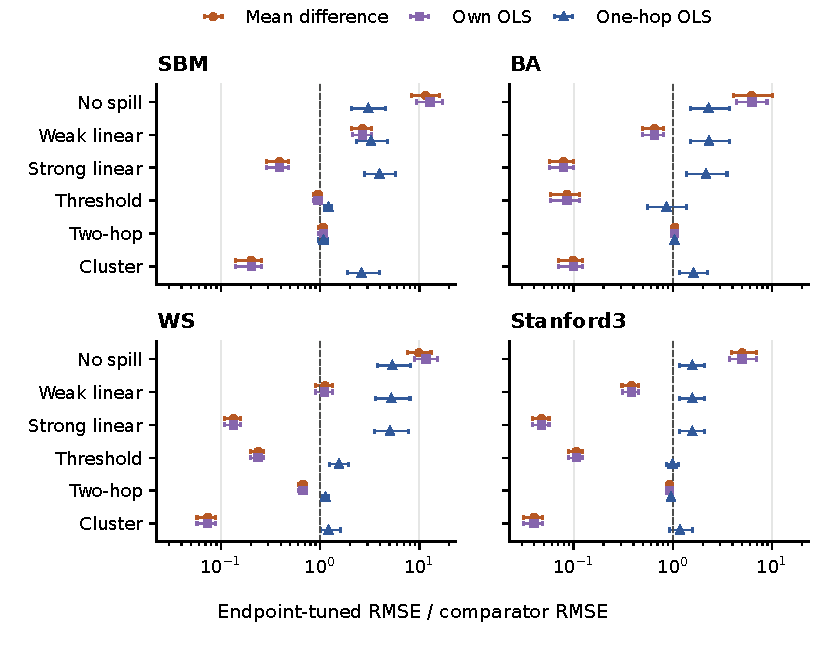
\includegraphics[width=\textwidth]{figures/conditional_accuracy.pdf}
\caption{Condition-specific accuracy across network families. Each point is the endpoint-tuned cell RMSE divided by a comparator's cell RMSE; values below one favor endpoint tuning. Bars are 95\% seed-block bootstrap intervals on a logarithmic horizontal axis. The same seed draws generate all ratios. Adding spillover adjustment helps relative to assignment-only estimators in strong-linear and cluster conditions, but the linear exposure-aware comparator is usually better.}
\label{fig:accuracy}
% @evidence[[analysis/summary.json#/ratios]] @evidence[[analysis/summary.json#/ratio_ci]]
\end{figure}

\subsection{Condition Heterogeneity and Misspecification}
The no-spill condition penalizes unnecessary flexibility. Endpoint-tuned RMSE ranges from 0.095 on Stanford3 to 0.594 on SBM, whereas difference-in-means RMSE ranges from 0.019 to 0.051. Even one-hop OLS pays for estimating an unnecessary exposure coefficient here. This comparison does not show that covariate adjustment is generally harmful: the complete references and targets differ, and it is confined to these realized noise, assignment, and topology settings.
% @evidence[[analysis/summary.json#/cell_rmse]]

Under strong linear spillover with individual assignment, difference-in-means RMSE is approximately two across families, reflecting the large global spillover contribution absent from its arm contrast. Endpoint tuning reduces these errors to 0.773, 0.158, 0.269, and 0.095 for SBM, BA, WS, and Stanford3, respectively. However, one-hop OLS is still better in every family, with corresponding RMSEs 0.194, 0.073, 0.053, and 0.061. Because this condition is linear in the exposure used by OLS, it is a particularly informative simple comparator. A flexible reference and a target-aware objective are not substitutes for a favorable specification.
% @evidence[[analysis/summary.json#/cell_rmse]]

Threshold spillovers expose strong structural heterogeneity. Endpoint-tuned RMSE is 2.373 on SBM, compared with 0.215 on BA, 0.592 on WS, and 0.265 on Stanford3. Its SBM signed bias is $-2.284$. One-hop OLS also has a large SBM threshold RMSE, 1.947, so this is not solely a weakness of the tuning rule. The threshold mechanism is outside the smooth quadratic reference. Sparse or concentrated observed exposure can make the unobserved part of this response important for the global contrast, but the recorded summaries do not isolate support as the cause of the error difference.
% @evidence[[analysis/summary.json#/cell_rmse]] @evidence[[analysis/summary.json#/cell_signed_bias]]

Under two-hop spillover, both exposure regressions are misspecified. Endpoint-tuned RMSE is 2.085 on SBM, 1.905 on BA, 1.209 on WS, and 1.802 on Stanford3; the corresponding signed biases are $-1.994$, $-1.899$, $-1.179$, and $-1.799$. One-hop OLS likewise has large errors. The global target includes an exposure pathway that the fitted one-hop model omits. Although observed one-hop exposure can correlate with two-hop exposure, this does not ensure accurate prediction when the entire assignment vector changes. The result supports a warning about this omitted mechanism, not a theorem that all one-hop regressions must fail or that any particular multi-hop replacement would succeed.
% @evidence[[analysis/summary.json#/cell_rmse]] @evidence[[analysis/summary.json#/cell_signed_bias]]

\subsection{Observed Fit and Assignment Design}
Figure~\ref{fig:diagnostics}(a) shows that observed-fit residual RMSE lies between 0.976 and 1.081 across all scientific records, close to the unit noise scale, while endpoint errors can be substantial. Threshold and two-hop cases occupy this same narrow residual range. An in-sample residual diagnostic therefore cannot be read as a certificate of accurate global prediction. This is a descriptive contrast, not an estimated causal relationship between residuals and endpoint error; records within a seed are dependent.
% @evidence[[analysis/summary.json#/fit_rmse_range]] @evidence[[analysis/observations.csv]]

\begin{figure}[t]
\centering
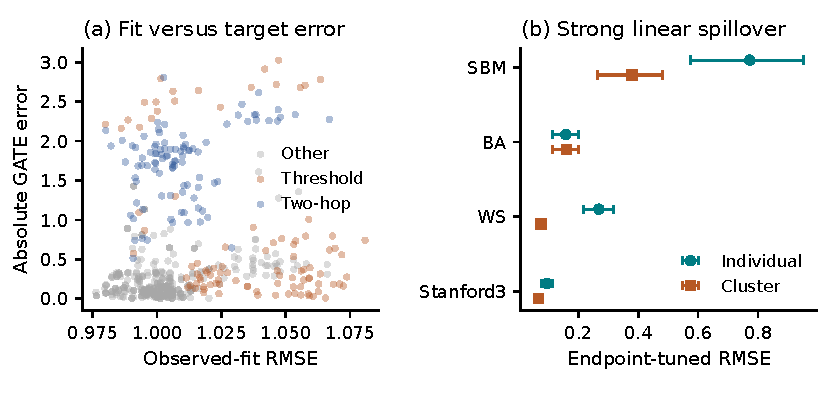
\includegraphics[width=\textwidth]{figures/diagnostic_limits.pdf}
\caption{Two limits of observed-data assessment. (a) Near-unit fitted residuals coexist with substantial absolute global-effect errors; all scientific records are shown, not independent graph samples. (b) For the same strong-linear outcome form, individual and cluster assignment yield different endpoint-tuned RMSEs across families. Bars are 95\% seed-block intervals. This design contrast changes the joint assignment distribution, not just one isolated exposure statistic.}
\label{fig:diagnostics}
% @evidence[[analysis/observations.csv]] @evidence[[analysis/summary.json#/cell_rmse_ci]]
\end{figure}

The cluster design reduces endpoint-tuned RMSE from 0.773 to 0.380 on SBM, from 0.269 to 0.075 on WS, and from 0.095 to 0.067 on Stanford3; BA changes from 0.158 to 0.160. These are point summaries, not claims that every design effect is significant. One-hop OLS remains better in all cluster cells. Exposure endpoint fractions increase especially on WS, where their seed-mean values change from 0.0014/0.0015 at zero/one under individual assignment to 0.1096/0.0917 under cluster assignment. Yet clustering changes treatment dependence and other aspects of the design simultaneously. We cannot attribute its performance differences solely to endpoint support or conclude that this clustering rule is optimal.
% @evidence[[analysis/summary.json#/cell_rmse]] @evidence[[analysis/summary.json#/support]]

\section{Discussion and Limitations}
\paragraph{What determines error within this study?}
The comparisons implicate an interaction between the estimator's reference, the interference mechanism, and the assignment distribution. Correctly represented strong linear spillovers favor a simple exposure-aware model over assignment-only analysis. Omitted two-hop spillovers leave large bias in both exposure regressions. A discontinuous response produces markedly different errors across families. These are controlled comparisons of evaluated configurations and prespecified outcome conditions, but not controlled manipulations of every graph property. Degree distribution, community structure, sample size, and exposure support vary together across families. Their isolated causal contributions are not estimated.

\paragraph{Target awareness is not endpoint validation.}
The reference risk calculation concerns noise within an adequate linear model. It cannot detect every discrepancy between that model and the endpoint response. Row-space membership ensures that the reference contrast has an algebraic representation in observed design coordinates; it does not demonstrate observations near all-treated and all-control assignments. Moreover, the selected criterion minimum is subject to reuse of the same outcomes. Neither a recorded small residual nor a finite selected estimate supplies the missing scientific guarantee. We do not claim empirical calibration of the risk criterion because selected penalties, contrast-weight norms, and fallback frequencies were not recorded.

\paragraph{Scope of uncertainty and reproducibility.}
The seed-block bootstrap preserves the paired structure of the evaluation but is based on a limited number of repeated realizations. The fixed Stanford3 graph supports a semi-synthetic topology-specific statement, not external validity for real platform outcomes. All outcomes are generated under the recorded mechanisms and noise scale. There are no confidence-interval coverage measurements, alternative noise stress studies, independently controlled tuning ablations, or evaluations of neural estimators. Absence of usable results for an alternative estimator supplies no evidence of inferior performance. The inspected source and evaluation records are available for audit; association through the selection manifest is not an independently reconstructed executable-identity proof.

\paragraph{Integrity and qualification.}
The final evaluation reports completion and successful task-specific qualification. Constant-outcome, node-relabeling, and reset-replay controls assess limited behavioral properties; their success is not evidence of statistical superiority, arbitrary-interference validity, or model identification. Candidate-produced internal diagnostics are unverified. We rely on evaluator-recorded estimates and retain the negative accuracy comparisons independently of this qualification outcome. Diagnostics not supplied by the evaluator remain unknown.
% @evidence[[paper_data.json#/grounding_sources/final.qualification.status]] @evidence[[paper_data.json#/grounding_sources/final.qualification.outcome]] @evidence[[paper_data.json#/final_evaluation/evaluation_evidence/candidate_diagnostics_trust]]

\paragraph{Reading the support diagnostics.}
An exposure endpoint fraction is a marginal summary across nodes in one realized assignment. It is not the probability of observing a global intervention, nor does it establish that every node's relevant response is represented. In the reference used here, own treatment and its interactions with exposure also enter the contrast. Observing exposure extremes without the relevant joint treatment configurations would not by itself validate those interaction predictions. The recorded linear-design condition number answers a different algebraic question from conditioning of the quadratic reference. Likewise, observed residuals mix noise with discrepancies near the experimental assignments; they cannot reveal a discrepancy confined to assignments not observed. These distinctions explain why the supplied diagnostics are useful warnings rather than a general selection rule. A practitioner would need scientifically justified exposure restrictions or additional experimental support before translating a favorable local fit into a reliable global deployment estimate. The present comparison quantifies the consequences for the specified cases, without measuring those additional requirements.
% @evidence[[source_evidence/estimator.py#L83-L160]] @evidence[[analysis/summary.json#/support]]

\section{Conclusion}
Global-effect estimation under interference is a contrast-prediction problem, and good observed fitting does not resolve it. In the evaluated network and outcome conditions, endpoint-tuned one-hop regression improves substantially on assignment-only estimators in several spillover settings but performs worse in aggregate than linear one-hop OLS. Reporting only the assignment-only comparisons would therefore overstate the evidence for a more elaborate target-aware estimator.

The most consequential failure cases combine endpoint prediction with either a threshold response or omitted two-hop exposure. A fixed-design risk rationale and algebraic estimability guards do not remove those specification limitations. Cluster assignment changes accuracy in a graph-dependent way, without isolating support as its sole cause. The practical lesson is to match the comparison to the target: use meaningful exposure-aware baselines, examine condition-specific bias and RMSE, and separate residual fit from endpoint accuracy. Controlled reference-matched tuning comparisons, explicit multi-hop adjustments, and repeated evaluations under additional noise and topology settings are needed before recommending this tuning rule more broadly. These are open empirical requirements, not results established by the present study.

\clearpage
\bibliography{references}
\bibliographystyle{source_evidence/iclr2026_conference}
\clearpage
\appendix
\section{Supplementary Information}
\subsection{Complete Condition-Level Accuracy}
Table~\ref{tab:cells} reports all scientific cells. Each entry uses the same 24 seeds and the estimand in Equation~\ref{eq:target}. Bias is signed for the endpoint-tuned estimator in this table, unlike the absolute-bias aggregate in the main text. Large negative values under two-hop interference reflect underestimation within these simulations. These entries are recomputed from the recorded estimates, not additional scientific evaluations.
% @evidence[[analysis/summary.json#/cell_rmse]] @evidence[[analysis/summary.json#/cell_signed_bias]]
\begin{table}[h]
\centering\small
\caption{Complete cell RMSEs and endpoint-tuned signed bias. ET: endpoint-tuned; DM: difference in means; Own: own-treatment OLS; Hop: one-hop OLS. All quantities are in outcome units.}
\label{tab:cells}
\begin{tabular}{llrrrrr}
\toprule Family & Condition & ET & DM & Own & Hop & ET bias\\\midrule
SBM & No spill & .594 & .051 & .046 & .194 & $-.043$\\
 & Weak linear & .632 & .237 & .235 & .194 & $-.098$\\
 & Strong linear & .773 & 1.982 & 1.982 & .194 & $-.184$\\
 & Threshold & 2.373 & 2.482 & 2.482 & 1.947 & $-2.284$\\
 & Two-hop & 2.085 & 1.940 & 1.940 & 1.919 & $-1.994$\\
 & Cluster & .380 & 1.877 & 1.874 & .145 & $-.085$\\\midrule
BA & No spill & .168 & .027 & .027 & .073 & $-.065$\\
 & Weak linear & .169 & .258 & .260 & .073 & $-.066$\\
 & Strong linear & .158 & 2.012 & 2.015 & .073 & $-.053$\\
 & Threshold & .215 & 2.511 & 2.513 & .249 & $-.095$\\
 & Two-hop & 1.905 & 1.821 & 1.823 & 1.825 & $-1.899$\\
 & Cluster & .160 & 1.623 & 1.623 & .099 & $-.069$\\\midrule
WS & No spill & .285 & .029 & .024 & .053 & $-.128$\\
 & Weak linear & .277 & .248 & .249 & .053 & $-.121$\\
 & Strong linear & .269 & 1.997 & 1.998 & .053 & $-.108$\\
 & Threshold & .592 & 2.494 & 2.495 & .380 & $-.503$\\
 & Two-hop & 1.209 & 1.797 & 1.798 & 1.065 & $-1.179$\\
 & Cluster & .075 & 1.025 & 1.026 & .062 & $.006$\\\midrule
Stanford3 & No spill & .095 & .019 & .019 & .061 & $-.001$\\
 & Weak linear & .095 & .250 & .251 & .061 & $-.001$\\
 & Strong linear & .095 & 2.000 & 2.000 & .061 & $-.002$\\
 & Threshold & .265 & 2.500 & 2.500 & .267 & $-.243$\\
 & Two-hop & 1.802 & 1.956 & 1.956 & 1.877 & $-1.799$\\
 & Cluster & .067 & 1.688 & 1.689 & .057 & $-.009$\\
\bottomrule\end{tabular}
% @evidence[[analysis/summary.json#/cell_rmse]] @evidence[[analysis/summary.json#/cell_signed_bias]]
\end{table}

\subsection{Exposure Support and Residual Diagnostics}
Table~\ref{tab:support} summarizes the exposure diagnostics for the matched strong-linear outcome conditions. Minima and maxima are averages of within-realization exposure extremes; endpoint fractions are averages across seeds. The condition number is for the evaluator's simple linear exposure design, not the selected quadratic design. Neither endpoint fractions nor this condition number certifies target identifiability. For Stanford3, endpoint exposures among a minority of nodes do not imply exposure support for every node or subgroup. Full recorded diagnostics are retained in \texttt{analysis/summary.json}.
\begin{table}[h]
\centering\small
\caption{Seed-mean observed exposure summaries. Ind.: individual assignment; Clust.: cluster assignment. $p_0,p_1$ are fractions of nodes with exposure exactly zero or one; $\kappa$ is the recorded linear-design condition number.}
\label{tab:support}
\begin{tabular}{llrrrrr}\toprule
Family & Design & Minimum & Maximum & $p_0$ & $p_1$ & $\kappa$\\\midrule
SBM & Ind. & .2372 & .7693 & .0000 & .0000 & 19.02\\
 & Clust. & .0170 & .9822 & .0006 & .0005 & 13.26\\
BA & Ind. & .0000 & 1.0000 & .0127 & .0134 & 7.59\\
 & Clust. & .0000 & 1.0000 & .0274 & .0329 & 7.70\\
WS & Ind. & .0000 & .9965 & .0014 & .0015 & 8.81\\
 & Clust. & .0000 & 1.0000 & .1096 & .0917 & 6.68\\
Stanford3 & Ind. & .0000 & 1.0000 & .0324 & .0321 & 9.19\\
 & Clust. & .0000 & 1.0000 & .0489 & .0398 & 7.21\\\bottomrule
\end{tabular}
% @evidence[[analysis/summary.json#/support]]
\end{table}
The residuals in Figure~\ref{fig:diagnostics} are observed-assignment in-sample errors, not held-out predictive errors. Even a held-out error at the same assignment distribution would answer a different question from the global intervention contrast unless additional structure connected the two. We do not estimate that connection here.

\subsection{Estimator Specification and Conditional Risk Criterion}
The numerical rank threshold is $\max(n,p_*)\epsilon_{\rm mach}s_{\max}$ for the standardized non-intercept design with $p_*$ columns. The residual norm of the endpoint contrast outside the retained right-singular-vector span must be at most $10^{-8}\max(1,\|q\|)$. Residual degrees of freedom are $n-r-1$, including the estimated intercept. Nonfinite inputs, failed SVD, unestimable contrast, nonpositive residual degrees of freedom, or no finite risk score trigger the fallback. The fallback uses $[1,x_i^\top,z_i,e_i,(e_i-.25)_+,(e_i-.5)_+,(e_i-.75)_+,z_ie_i]$, ridge penalty $10^{-3}$ on non-intercept coefficients, and no intercept penalty. Exact equality of all outcomes invokes a constant predictor. These are inspectable source properties; no frequencies of their activation are available.
% @evidence[[source_evidence/estimator.py#L69-L81]] @evidence[[source_evidence/estimator.py#L119-L158]] @evidence[[source_evidence/estimator.py#L199-L213]]

For clarity, write $b_\lambda=a_\lambda^\top\mu_c-\gate$ under the correct reference. The fixed-penalty calculation is
\begin{align}
E[(\widehat\gate_\lambda-\widehat\gate_0)^2]
 &=b_\lambda^2+\sigma^2\|a_\lambda-a_0\|^2,\\
E[\widehat R(\lambda)]
 &=b_\lambda^2+\sigma^2\|a_\lambda\|^2.
\end{align}
The variance correction depends on the same contrast weights as the fitted endpoint predictions. These equations require an unbiased reference and variance estimate and concern a fixed rule conditional on the design. They neither justify reporting the selected minimum as unbiased nor establish an endpoint-risk calibration experiment. We did not record selected penalties, support probabilities, or contrast amplification distributions.
% @evidence[[source_evidence/estimator.py#L127-L151]]

\subsection{Benchmark Construction and Reproduction}
The exact archived inputs, rather than regenerated approximations, define this evaluation. Synthetic graphs use NetworkX 3.3 and PCG64 seeds given by the statistical seed plus $100003$ times the one-based family index. The statistical seeds are
\begin{quote}\small
1009, 1013, 1019, 1021, 1031, 1033, 1039, 1049, 1051, 1061, 1063, 1069, 1087, 1091, 1093, 1097, 1103, 1109, 1117, 1123, 1129, 1151, 1153, 1163.
\end{quote}
Graphs are normalized to unique undirected edges without self-loops, preserving the declared node set. Graph-specific noise is reused across the outcome conditions, and fitting never receives counterfactual outcomes. The supplied final manifest records graph and raw-row fingerprints. The benchmark archive contains the covariates, assignments, and observed outcomes needed to replay the comparison; a stand-alone raw-input generator is not supplied, so exact regeneration from prose alone is not claimed.
% @evidence[[source_evidence/benchmark_manifest.json#/seeds]] @evidence[[source_evidence/benchmark_manifest.json#/generator]] @evidence[[source_evidence/benchmark_manifest.json#/normalization]] @evidence[[reproducibility/resources/final/benchmark.npz]]

The declared research environment is NumPy 1.26.4, SciPy 1.13.1, and NetworkX 3.3 under Python 3.11 or 3.12. The evaluation allows at most two CPU cores and 8 GiB per role, with numerical library threads set to one. Its final wall-clock allowance is 7,200 seconds; the recorded complete evaluation elapsed time is about 629 seconds, not a per-estimator runtime. No comparative speed claim follows. A replay requires the evaluator's supported Linux isolation facilities. \texttt{REPRODUCIBILITY.md} records the checked entrypoints and distinguishes replay commands, which were not rerun for this manuscript, from the derived-analysis command that was executed.
% @evidence[[source_evidence/requirements.txt]] @evidence[[source_evidence/benchmark_manifest.json#/time_plan]] @evidence[[source_evidence/final_manifest.json#/compute_usage]]

Every quantitative figure and table is derived by \texttt{build\_paper\_artifacts.py} from \texttt{paper\_data.json}; the saved observation table and summaries retain their evidence trails. The required overview is conceptual and is rendered separately from the manuscript's figure specification. The public Stanford3 archive is attributed to \citet{Traud2012} and \citet{Rossi2015}. It was obtained from Network Repository as \texttt{socfb-Stanford3.zip}, with SHA-256 \texttt{b1221e414dbaf3278468f60881bac932e935b8813020157bc6fb3823f5e8720d}. The archive is distributed under the repository's stated CC BY-SA terms; redistribution must retain attribution and share-alike obligations. This is synthetic-outcome research on public topology, not an analysis of real experimental outcomes.
% @evidence[[source_evidence/evaluate_final.py#L729-L754]] @evidence[[source_evidence/benchmark_manifest.json#/attribution]]

Literature access was limited to the supplied permitted titles and direct classical statistical and graph-model sources. Title/abstract records and selected original documents are retained in \texttt{reference\_evidence/}. Citation graphs, related-content searches, and identification of the restricted study were not used. No restricted material was knowingly encountered in this paper-writing step. Reading scope is recorded per reference; the discussion does not rely on unread detailed results.

\subsection{Evaluation Integrity and Missing Evidence}
The authoritative final status is completed and the qualification outcome is qualified. The recorded control success fraction is one and failed-episode fraction is zero. Constant-outcome controls require zero endpoint contrast; node relabeling checks that predictions commute with a fixed nontrivial relabeling; reset replay checks repeated predictions after state clearing. These finite checks do not guarantee validity for every graph or mechanism. Internal estimator diagnostics are explicitly unverified in the evaluation record. Qualification is independent of whether a baseline is better, and our negative one-hop comparison remains part of the scientific conclusion.
% @evidence[[paper_data.json#/grounding_sources/final.qualification.status]] @evidence[[paper_data.json#/grounding_sources/final.qualification.outcome]] @evidence[[paper_data.json#/final_evaluation/metrics/control_success_fraction]] @evidence[[paper_data.json#/final_evaluation/metrics/failed_episode_fraction]] @evidence[[source_evidence/evaluate_final.py]]

No completed component ablation or matched final comparison to the original fixed-hinge configuration is available. A separate two-hop configuration lacks usable comparative measurements; its local failure record reports an evaluator disconnection, not a measured accuracy loss, and the underlying cause is unresolved. It is excluded from performance tables rather than assigned an artificial error. Hidden-endpoint twin simulations, empirical risk calibration, alternative-noise studies, and inference coverage studies were not performed. This missing evidence limits attribution and recommendations even though the fixed comparison is complete.
% @evidence[[source_evidence/missing_comparison_failure.json]] @evidence[[source_evidence/missing_comparison_stderr.log]]

\subsection{LLM Usage}
Large language models contributed to research framing, estimator proposals, code generation, literature-query planning, manuscript strategy, mathematical exposition, and writing. For the present manuscript, an LLM inspected the supplied source and evaluation artifacts, wrote the deterministic summary and plotting script, retrieved and read bounded permitted-source records, drafted the text and claim map, and iterated on validation. The quantitative analysis reaggregates existing evaluator-recorded observations; it does not replace them with generated measurements. The conceptual overview uses the separately orchestrated illustration workflow. No human-verification claim is made. Proposed but unexecuted studies are explicitly distinguished from measured results, and the role of model-assisted writing does not alter the scientific qualification or limitations.

\end{document}
